\phantomsection
\section{GMI SRF Data Plots}
%===========================
\label{app.srf_data_plots}

\addcontentsline{toc}{subsection}{Channels 1-3}
\begin{figure}[H]
  \centering
  \begin{tabular}{c c}
    \multicolumn{2}{c}{\sffamily\textbf{Channel 1}}\\
    \includegraphics[scale=0.35]{graphics/lin/gmi_gpm-1.eps} &
    \includegraphics[scale=0.35]{graphics/log/gmi_gpm-1.eps} \\
    \multicolumn{2}{c}{\sffamily\textbf{Channel 2}}\\
    \includegraphics[scale=0.35]{graphics/lin/gmi_gpm-2.eps} &
    \includegraphics[scale=0.35]{graphics/log/gmi_gpm-2.eps} \\
    \multicolumn{2}{c}{\sffamily\textbf{Channel 3}}\\
    \includegraphics[scale=0.35]{graphics/lin/gmi_gpm-3.eps} &
    \includegraphics[scale=0.35]{graphics/log/gmi_gpm-3.eps}
  \end{tabular}
  \caption{GMI channels 1-3 responses for the three test temperatures: $T_{NOM}$ (25\textdegree{}C), $T_{LO}$ (-10\textdegree{}C), and $T_{HI}$ (45\textdegree{}C). Vertical dashed lines are the locations of the computed central frequencies. \textbf{(Left)} Linear y-axis. \textbf{(Right)} Base-10 logarithmic y-axis.}
  \label{fig:ch1-3_response}
\end{figure}

\addcontentsline{toc}{subsection}{Channels 4-6}
\begin{figure}[H]
  \centering
  \begin{tabular}{c c}
    \multicolumn{2}{c}{\sffamily\textbf{Channel 4}}\\
    \includegraphics[scale=0.35]{graphics/lin/gmi_gpm-4.eps} &
    \includegraphics[scale=0.35]{graphics/log/gmi_gpm-4.eps} \\
    \multicolumn{2}{c}{\sffamily\textbf{Channel 5}}\\
    \includegraphics[scale=0.35]{graphics/lin/gmi_gpm-5.eps} &
    \includegraphics[scale=0.35]{graphics/log/gmi_gpm-5.eps} \\
    \multicolumn{2}{c}{\sffamily\textbf{Channel 6}}\\
    \includegraphics[scale=0.35]{graphics/lin/gmi_gpm-6.eps} &
    \includegraphics[scale=0.35]{graphics/log/gmi_gpm-6.eps}
  \end{tabular}
  \caption{GMI channels 4-6 responses for the three test temperatures: $T_{NOM}$ (25\textdegree{}C), $T_{LO}$ (-10\textdegree{}C), and $T_{HI}$ (45\textdegree{}C). Vertical dashed lines are the locations of the computed central frequencies. \textbf{(Left)} Linear y-axis. \textbf{(Right)} Base-10 logarithmic y-axis.}
  \label{fig:ch4-6_response}
\end{figure}

\addcontentsline{toc}{subsection}{Channels 7-9}
\begin{figure}[H]
  \centering
  \begin{tabular}{c c}
    \multicolumn{2}{c}{\sffamily\textbf{Channel 7}}\\
    \includegraphics[scale=0.35]{graphics/lin/gmi_gpm-7.eps} &
    \includegraphics[scale=0.35]{graphics/log/gmi_gpm-7.eps} \\
    \multicolumn{2}{c}{\sffamily\textbf{Channel 8}}\\
    \includegraphics[scale=0.35]{graphics/lin/gmi_gpm-8.eps} &
    \includegraphics[scale=0.35]{graphics/log/gmi_gpm-8.eps} \\
    \multicolumn{2}{c}{\sffamily\textbf{Channel 9}}\\
    \includegraphics[scale=0.35]{graphics/lin/gmi_gpm-9.eps} &
    \includegraphics[scale=0.35]{graphics/log/gmi_gpm-9.eps}
  \end{tabular}
  \caption{GMI channels 7-9 responses for the three test temperatures: $T_{NOM}$ (25\textdegree{}C), $T_{LO}$ (-10\textdegree{}C), and $T_{HI}$ (45\textdegree{}C). Vertical dashed lines are the locations of the computed central frequencies. \textbf{(Left)} Linear y-axis. \textbf{(Right)} Base-10 logarithmic y-axis.}
  \label{fig:ch7-9_response}
\end{figure}

\addcontentsline{toc}{subsection}{Channels 10-12}
\begin{figure}[H]
  \centering
  \begin{tabular}{c c}
    \multicolumn{2}{c}{\sffamily\textbf{Channel 10}}\\
    \includegraphics[scale=0.35]{graphics/lin/gmi_gpm-10.eps} &
    \includegraphics[scale=0.35]{graphics/log/gmi_gpm-10.eps} \\
    \multicolumn{2}{c}{\sffamily\textbf{Channel 11}}\\
    \includegraphics[scale=0.35]{graphics/lin/gmi_gpm-11.eps} &
    \includegraphics[scale=0.35]{graphics/log/gmi_gpm-11.eps} \\
    \multicolumn{2}{c}{\sffamily\textbf{Channel 12}}\\
    \includegraphics[scale=0.35]{graphics/lin/gmi_gpm-12.eps} &
    \includegraphics[scale=0.35]{graphics/log/gmi_gpm-12.eps}
  \end{tabular}
  \caption{GMI channels 10-12 responses for the three test temperatures: $T_{NOM}$ (25\textdegree{}C), $T_{LO}$ (-10\textdegree{}C), and $T_{HI}$ (45\textdegree{}C). \textbf{(Left)} Linear y-axis. \textbf{(Right)} Base-10 logarithmic y-axis.}
  \label{fig:ch10-12_response}
\end{figure}

\addcontentsline{toc}{subsection}{Channel 13}
\begin{figure}[H]
  \centering
  \begin{tabular}{c c}
    \multicolumn{2}{c}{\sffamily\textbf{Channel 13}}\\
    \includegraphics[scale=0.35]{graphics/lin/gmi_gpm-13.eps} &
    \includegraphics[scale=0.35]{graphics/log/gmi_gpm-13.eps}
  \end{tabular}
  \caption{GMI channel 13 responses for the three test temperatures: $T_{NOM}$ (25\textdegree{}C), $T_{LO}$ (-10\textdegree{}C), and $T_{HI}$ (45\textdegree{}C). \textbf{(Left)} Linear y-axis. \textbf{(Right)} Base-10 logarithmic y-axis.}
  \label{fig:ch10-13_response}
\end{figure}
